\documentclass[a4paper,17pt]{article}

\usepackage[T2A]{fontenc}	
\usepackage[utf8]{inputenc}	
\usepackage[english,russian]{babel}
\usepackage{floatrow}
\usepackage{caption}
\usepackage{amsmath,amsfonts,amssymb,amsthm,mathtools}
\usepackage{wrapfig}
\usepackage[14pt]{extsizes} % для того чтобы задать нестандартный 14-ый размер шрифта



\title{Лабораторная работа №2.1.1\\
Измерение удельной теплоемкости воздуха при постоянном давлении}
\author{Дмитрий Павлов}
\date{Апрель 2018}
\thispagestyle{empty} % выключаем отображение номера для этой страницы

\begin{document}
\maketitle
\begin{center}	
    \textit{Московский физико-технический институт}
	\vspace{0.5ex} 
\end{center}

\textbf{Цель работы:} измерить повышение температуры воздуха в зависимости от мощности подводимого тепла и расхода при стационарном течении через трубу; исключив тепловые потери, по результатам измерений определить теплоёмкость воздуха при постоянном давлении.\\

\textbf{В работе используются:} 
\begin{itemize}
    \item теплоизолированная стеклянная трубка,
    \item электронагреватель,
    \item источник питания постоянного тока,
    \item амперметр, вольтметр (цифровые мультиметры)
    \item термопара, подключенная к микровольтметру,
    \item компрессор,
    \item газовый счётчик,
    \item секундомер
\end{itemize}

\newpage

\section{Теоретическая справка}

    Теплоёмкость тела в некотором процессе определяется как их отношение:
    
    %Формула теплоемкость
    \begin{equation}
        C = \frac{\delta Q}{\Delta T}
    \end{equation}
        
    Надёжность измерения определяется, в основном, качеством калориметра. Необходимо, чтобы количество тепла, затрачиваемое на нагревание исследуемого тела, существенно превосходило тепло, расходуемое на нагревание самого калориметра, а также на потери тепла из установки Для увеличения количества нагреваемого газа при неизменных размерах установки воздух продувается через калориметр, внутри которого установлен нагреватель. При этом измеряются мощность нагревателя, масса воздуха, протекающего в единицу времени, и приращение его температуры.
    
    \begin{center}
        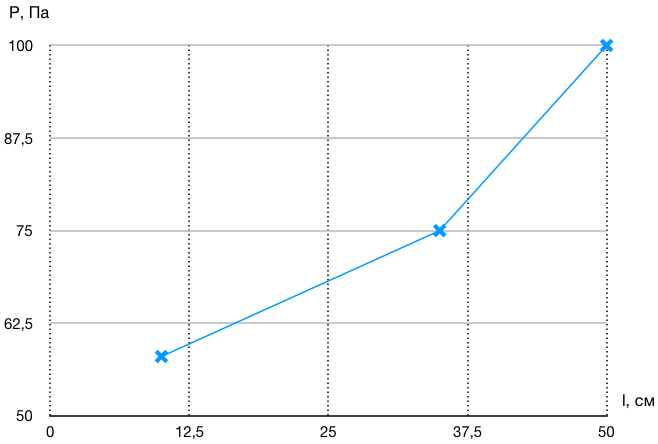
\includegraphics[scale = 0.6]{q3.png}\\    
    \end{center}
    
    Рассмотрим газ, протекающий стационарно слева направо через трубу постоянного сечения, в которой установлен нагревательный элемент (см. рис.). Пусть за некоторое время $d t$ через калориметр прошла малая порция газа массой $d m = q d t$, где $q$ [кг/с] — массовый расход газа в трубе. Если мощность нагрева равна  $N$, мощность тепловых потерь на обмен с окружающей средой $N_1$, то порция получила тепло $\delta Q = (N - N_1)d t$. C другой стороны, по определению теплоемкости: $\delta Q = c d m \Delta T$, где $\Delta T = T_2 - T_1$ - приращение температуры газа, и $с$ - удельная (на единицу массы) теплоемкость газа в рассматриваемом процессе. При малых расходах газа и достаточно большом диаметре трубы перепад давления на её концах мал, поэтому можно принять, что $P_1 \approx P_2 = P_0$, где $P_0$ - атмосферное давление. Следовательно, в условиях опыта измеряется удельная теплоемкость при постоянном давлении $c_p$. Таким образом, получаем:
    
    %Итоговая формула
    \begin{equation}
        c_p = \frac{N - N_1}{q \Delta T}\label{answer}
    \end{equation}

\subsection{Экспериментальная установка}
    Воздух, нагнетаемый компрессором, прокачивается через калориметр. Калориметр представляет собой стеклянную цилиндрическую трубку с двойными стенками, запаянными с торцов. На внутреннюю поверхность стенок трубки нанесено серебряное покрытие для минимизации потерь тепла за счет излучения. Воздух из пространства между стенками калориметра откачан до высокого вакуума (5-10 торр) для минимизации потерь тепла, обусловленных теплопроводностью.
    
    \begin{center}
        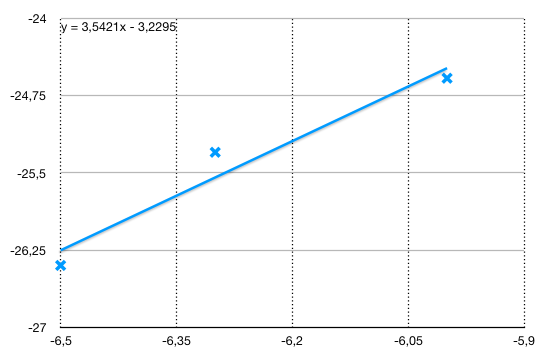
\includegraphics[scale = 0.7]{q4.png}   
    \end{center}
    
    Для измерения разности температур $\Delta T$ служит медно-константановая термопара. Один спай термопары расположен в струе воздуха, входящего в калориметр, и находится при комнатной температуре, а второй в струе выходящего нагретого воздуха.
    Коэффициент пропорциональности между ЭДС на термопаре и разностью температур в трубке:
    
    \begin{equation}
        \beta = \frac{E}{\Delta T} = 40.7 \frac{mkV}{^\circ C} \label{betta}
    \end{equation}
    
    \begin{center}
        где $E$ - ЭДС на термопаре, $\Delta T$ - разность температур    
    \end{center}
    
    ЭДС регистрируется с помощью микровольтметра. Объем воздуха, прошедшего через калориметр, измеряется газовым счетчиком ГС. Для регулировки расхода служит кран К.
    
    Объемный расход равен $\Delta V/ \Delta t$, массовый расход может быть найден как
    
    \begin{equation}
        q=\rho_0\frac{\Delta V}{\Delta t}\label{rash}
    \end{equation}
    
    где $\rho_0$ — плотность воздуха при комнат- ной температуре, которая в свою очередь может быть получена из уравнения Менделеева–Клапейрона:
    
    \begin{equation}
        \rho_0=\frac{\mu P_0}{RT_0}\label{rho}
    \end{equation}
          
\section{Ход работы}

    \begin{itemize}
        \item Используя термометр, определим температуру и влажность воздуха. С помощью этих данных, определим значение $C_P$ для воздуха.
        \item Измерим объемный расход воздуха при максимально открытом кране.
        \item Посчитаем мощность нагревателя, приняв значения сопротивления проволоки (которая используется в нагревателе) $\approx$ 35 Ом.
    \end{itemize}
        
    \subsection{Теоретическая оценка $C_P$ воздуха:}
        Температура: $26^\circ$C\\
        Давление: $100600$ Па\\
        Влажность: 63\%
        
        По этим данным определим плотность воздуха, пользуясь уравнением \ref{rho}:
        \begin{center}
            $\rho_0=\frac{\mu P_0}{RT_0} = 1.17$ кг/м$^3$\label{rho_res} 
        \end{center}
           
        
        Теплоемкость двухатомного газа находится так:
        \begin{center}
            $C_P = \frac{7R}{2}=$ 29 Дж/моль$\cdot$К    
        \end{center}
            
        
    \subsection{Максимальный поток воздуха:}       
        Настроим подачу воздуха к установке, измерим максимальный поток воздуха:
        
        \begin{center}
            \begin{tabular}{ | l | l |}
                \hline
                $\Delta V / \Delta t$, л/c & q, г/с \\ \hline
                0.11    &   0.13 \\
                0.11    &   0.13 \\
                0.11    &   0.13 \\
                \hline
            \end{tabular}
            
        $\Delta V / \Delta t$ измерено с помощью газового счетчика
        \end{center}        
        Расход q рассчитывается по формуле (\ref{rash}), плотность $\rho$ = 1.17 кг/м$^3$ посчитана выше.
        
\newpage
\section{Измерение зависимость разности температур от мощности нагревателя при максимальном расходе воздуха.}
    Масса воздуха m, протекающего через калориметр в секунду, рассчитывается по расходу воздуха, измеренного счетчиком.
    
    q = 0.13 г/c, $\Delta t$ = 45 c
    
    m = 8.5 $\cdot 10^{-5}$ кг
    
    \subsection{Результаты измерения ЭДС на термопаре при максимальном потоке воздуха}
    
    Напряжение подается на нагревательный элемент, который создает разность температур между воздухом внутри калориметра и воздухом снаружи.
    Дождемся пока режим установится (прекратится рост ЭДС термопары).
    
        \begin{center}
            \begin{tabular}{ | l | l | l |}
                \hline
                I, мА & U, В & $\varepsilon$, мВ \\ \hline
                89      &   3       &   80  \\
                120.7   &   4.083   &   153 \\
                139.6   &   4.725   &   210 \\
                155.8   &   5.274   &   266 \\
                178.6   &   6.046   &   350 \\
                \hline
            \end{tabular}\\
            
            ЭДС на термопаре в зависимости от поданного напряжения
        \end{center}
    
    \subsection{Из данных предыдущей таблицы вычислим $\Delta T$ и $N$:}
    Воспользуемся зависимостью (\ref{betta}), связывающей ЭДС на термопаре и разность температур. По известной формуле вычислим мощность цепи N.
    
        \begin{center}
            \begin{tabular}{ | l | l | l | l | l |}
                \hline
                I, мА & U, В & $\varepsilon$, мВ & $\Delta T, K$ & N, Вт\\ \hline
                89      &   3       &   80  &   1.97    &   0.267\\
                120.7   &   4.083   &   153 &   3.75    &   0,493\\
                139.6   &   4.725   &   210 &   5.16    &   0,658\\
                155.8   &   5.274   &   266 &   6.53    &   0,822\\
                178.6   &   6.046   &   350 &   8.6     &   1,078\\
                \hline
            \end{tabular}\\
            
            ЭДС на термопаре и разность температур связаны уравнением: $\varepsilon = \beta \cdot \Delta T$
        \end{center}
        
\section{Измерение зависимость разности температур от мощности нагревателя при меньшем  расходе воздуха.}
    Аналогично пункту 3 вычислим массу проходящего воздуха:

    m = 6.8 $\cdot 10^{-5}$ кг
    
    \subsection{Измерение ЭДС на термопаре при меньшем потоке}
    
        \begin{center}
            \begin{tabular}{ | l | l | l |}
                \hline
                I, мА & U, В & $\varepsilon$, мВ \\ \hline
                44.9    &   1.513   &   30  \\
                77.1    &   2.602   &   102 \\
                104.4   &   3.69    &   216 \\
                142.5   &   4.822   &   368 \\
                175.1   &   5.929   &   565 \\
                \hline
            \end{tabular}\\
            ЭДС на термопаре в зависимости от поданного напряжения
        \end{center}
        
    \subsection{По ЭДС на термопаре вычислим $\Delta T$ и $N$:}
    
        \begin{center}
            \begin{tabular}{ | l | l | l | l | l |}
                \hline
                I, мА & U, В & $\varepsilon$, мВ & $\Delta T, K$ & N, Вт\\ \hline
                44.9    &   1.513   &   30      &   0.73    &   0.068   \\
                77.1    &   2.602   &   102     &   2.51    &   0.2     \\
                104.4   &   3.69    &   216     &   5.31    &   0.385   \\
                142.5   &   4.822   &   368     &   9.04    &   0.687   \\
                175.1   &   5.929   &   565     &   13.9    &   1.038   \\
                \hline
            \end{tabular}\\
            
            ЭДС на термопаре и разность температур связаны уравнением: $\varepsilon = \beta \cdot \Delta T$
        \end{center}
        
\newpage
\section{Построение графиков зависимостей $T(E)$.}
    Учитывая уравнение \ref{answer} ожидаем зависимость N($\Delta t$) линейной. Коэффициент наклона равен теплоемкости воздуха.
    \begin{center}
        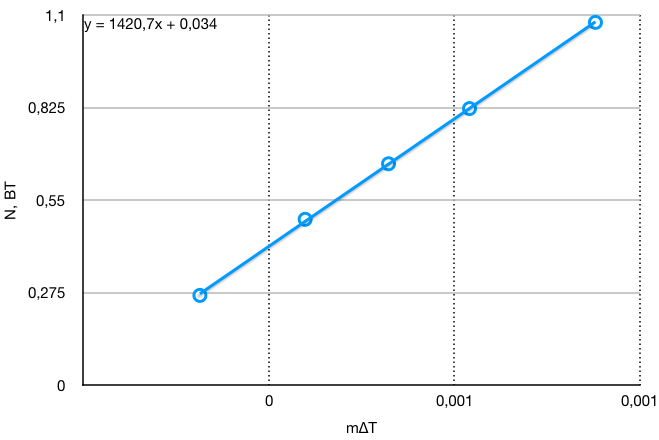
\includegraphics[scale = 0.6]{q1.png}\\
        График зависимости разности температур на концах трубки от ЭДС нагревателя при максимальном расходе воздуха.\\
        Коэффициент наклона прямой k = 1420
    \end{center}
    
    \begin{center}
        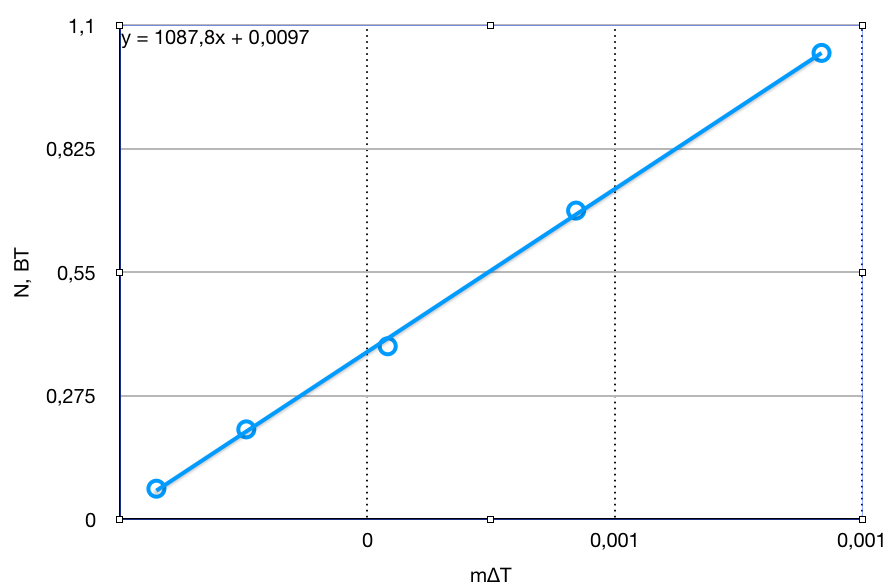
\includegraphics[scale = 0.45]{q2.png}\\
        График зависимости разности температур на концах трубки от ЭДС нагревателя при меньшем расходе воздуха.\\
        Коэффициент наклона прямой k = 1090
    \end{center}
    Разница в углах наклона объясняется разным качеством опытов: в первом случае через установку проходило больше воздуха и следовательно теплопотери сказываются меньше.
    \subsection{Найдем $c_p$:}
    
        \begin{center}
            $c_{p1}$ = 1420 Дж/кг$\cdot$К                   \\ 
            $c_{p2}$ = 1090 Дж/кг$\cdot$К                   \\
            $c_{p}$ = 1250 $\pm$ 200 Дж/кг$\cdot$К          \\
            $\varepsilon(c_p)$ =  15 \%                     \\
            Теоретическое $c_{p}$ = 1005 Дж/кг$\cdot$К      \\
            Табличное значение: $c_{p}$ = 1119 Дж/кг$\cdot$К\\
        \end{center}
        
    \subsection{Погрешности:}
    
        \subsubsection{Систематическая погрешность:}
            
            \begin{itemize}
                \item 
                    $q=\rho_0\frac{\Delta V}{\Delta t}, $
                    $\rho_0=\frac{\mu P_0}{RT_0}$ (см. теоретическую справку), т.е.
                    
                \begin{center}
                    $\sigma(q) = q\sqrt{(\frac{\sigma(\Delta t)}{\Delta t})^2 + (\frac{\sigma(V)}{V})^2 + (\frac{\sigma(P)}{P})^2 + (\frac{\sigma (\Delta T)}{\Delta T})^2}$ =
                    
                    = 0.13$\sqrt{(\frac{0.1}{45})^2 + (\frac{0.1}{8})^2 + (\frac{1}{100000})^2 + (\frac{0.25}{5})^2} = 0.13 \cdot 0.1 = 0.013$ г/с
                \end{center}
                
                \item 
                $T = E / \beta$, считаем, что $\beta$ = 0.0407 В/$^\circ C$ точно, таким образом: 
                
                \begin{center}
                     $\sigma(T) = \frac{\sigma(E)}{\beta} \approx \frac{0.01}{0.04} = 0.25$ 
                \end{center}
                
                \item
                $N = IU$, т.е.     
                
                \begin{center}
                    $\sigma(N) = N\sqrt{(\frac{\sigma(I)}{I})^2 + (\frac{\sigma(U)}{U})^2} = 0.55\cdot \sqrt{(\frac{0.01}{0.1})^2+(\frac{0.01}{3})^2} = 0.05$
                \end{center}
                
            \end{itemize}
            
                        \begin{center}
                \begin{tabular}{ | l | l | l |}
                    \hline
                    Погрешность величины& значение  &   причины                 \\ \hline
                    $\sigma (\Delta V)$ &   0.1л    &   точность ГС             \\
                    $\sigma (I)$        &   0.01А   &   точность амперметра     \\
                    $\sigma (E)$        &   0.01В   &   точность вольтметра     \\
                    $\sigma (\Delta t)$ &   0.1c    &   реакция человека        \\
                    $\sigma (T)$        &   0.25К   &   косвенная погрешность   \\
                    $\sigma (N)$        &   0.05Вт  &   косвенная погрешность   \\
                    $\sigma (q)$        &   0.013   &   косвенная погрешность   \\
                    \hline
                \end{tabular}   
            \end{center}
            
            Таким образом, систематическая погрешность измерения теплоемкости равна:
            
            \begin{center}
                $c_p \approx \frac{N}{q \Delta T}$
            
                $\sigma(c_p) = c_p\sqrt{(\frac{\sigma(N)}{N})^2 + (\frac{\sigma(q)}{q})^2 + \frac{\sigma(\Delta T)}{\Delta T})^2}$ =
                
                = $1250\sqrt{(\frac{0.05}{55})^2 + (\frac{0.013}{0.13})^2 + (\frac{0.25}{5})^2}$ = $1250 \cdot 0.15$ = 187 
            \end{center}
            
        \subsubsection{Случайная погрешность:}
        
            Случайная погрешность, погрешность углового коэффициента:
    
            \begin{center}
                $\sigma_{k} = \frac{1}{\sqrt{n}}\sqrt{\frac{\langle y^2 \rangle - \langle y \rangle ^2}{\langle x^2 \rangle - \langle x \rangle ^2} - k^2}$
            \end{center}
            
            Получаем значение $k = \frac{P}{\Delta T} = 0.165 \pm 0.005$
            То есть случайная погрешность $\approx$ 60 Дж/кг$\cdot$К
        \subsubsection{Итоговая погрешность:}
            \begin{center}
                $\sigma(c_p) = \sqrt{60^2 + 187^2} = 196 \approx 200$ Дж/кг$\cdot$К
            \end{center}
    
\section{Вывод}
    Табличное значение $c_p$ совпало со значением, полученным во время опыта в пределах погрешности. Погрешность составила 15\%. Основной причиной возникновения ошибки является непостоянное давление поступающего воздуха, а значит и расход Q. Также оказало влияние непостоянная температура вокруг установки.
\end{document}
    
